




\documentclass[12pt]{article}
\usepackage[utf8]{inputenc}
\usepackage[T1]{fontenc}
\usepackage{color}
\usepackage{graphicx}
\usepackage[top=3cm,bottom=2cm,left=3cm,right=2cm]{geometry}
\special{papersize=210mm,297mm}

\usepackage[citecolor=cyan,colorlinks,linkcolor=blue]{hyperref}
\usepackage{aeguill} 

\newcommand{\df}{\emph{modèle Dataflow}}
\newcommand{\imp}{\emph{modèle Impératif}}
\newcommand{\hll}{\emph{HyperLogLog}}

\begin{document}
\nocite{*}
\begin{center}
   {\Large\textbf{HyperLogLog Implementation}}
\medskip \\
   {\large  Nicolas Lupinski \& Rémy El Sibaïe Besognet}
\end{center}

\medskip\noindent

\medskip \noindent

\newpage

\tableofcontents

\newpage

\section{Introduction}

\hll\ is an efficient algorithm for cardinality estimation. The first
draft of this algorithm was proposed by P. Flajolet \& \emph{al} in
the 90s. We study and implement here a practical version from Google
Engineers \cite{HeuleNH13}.  This realisation was part of an
algorithmic course (GRAAL) teached by Michèle Soria and Fabien Viger.

In section 2, we present the original version of \hll. In section 3,
we give details on the different phases of implementation and
optimisation, and how we approach them. We conclude then with details
about our organisation, opinions and experiences about this course.

\section{Original work on \hll}

\hll\ can approximate counting efficiently thanks to a few properties
of hash function. First, two distinct object have distinct hashed values with
extremely high probability, so one can count the number of distinct
hash intead of the original objects. Second, hashed values are
distributed uniformaly. There is multiple way this property can be used
to approximate counting, \hll\ use this one: the probability of
finding $n$ leading zeros in the hashed value is $2^{-n}$. Hence,
finding a hashed value with $n$ leading zeros let us estimate there is
$2^{n}$. \hll\ only have to store $\rho$ the highest number of leading zeros
in order to perform an estimation, which is a small integer of size
$log h$ where h is the size of the hash function. Hence $\rho$ can be
coded on $log(log(h))$ bits.

In order to increase the accuracy of the estimate (a single estimator
can only at best gives the magnitude of the cardinality), we want to
use more than a single hash function, and merge the result in some
way. This can be done straightforwardly by splitting the original hash
value in two : the first $p$ bits are considered to be an index, and
the remaining bits are an hash value (of which we count the number of
leading zeros). \hll\ memorizes $2^{p}$ values to perform it's
estimations, and the new estimator is their average times $2^{p}$.



\section{Implementation and optimizations}

\subsection{First draft of the implementation}

We choosed to implement \hll in Ocaml. Our first 32 bits
implementation was pure Ocaml. When we upgraded to 64 bits hash
functions, we used an external C library to get a fast hash and a fast
count of the number of leading zeros. We start benchmarking by
counting the time spent by a set of 10000000 elements. The average
time to execute \texttt{Hll.add} is $30ms$ while \texttt{C++} takes
$1.5ms$, even with the underlying \texttt{C} implementation for the
number of leading zeros and the hash function.


\begin{figure}[h!]
   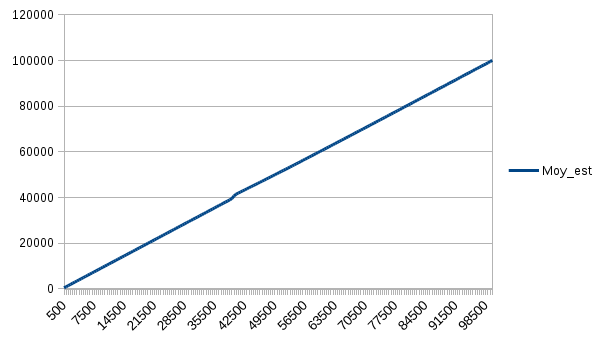
\includegraphics[scale=1]{./moy.png}
   \caption{\label{figmoy}Estimate average}
  
\end{figure}

The first experimentation is to run 1000 times the algorithm on random
data of cardinality from 500 to 100000. From this, we obtained figure
\ref{figmoy} with represent the effective cardinality on the y-axis and
the exact cardinality on x-axis.
We can observe a small bump at $n=40000$ which represent the switch
from $LinearCounting$ to \hll.
The error seems small but if we plot the average relative error in
percent we observe a pike at $2.5\%$ decreasing quickly from $40000$.

\begin{figure}[h!]
   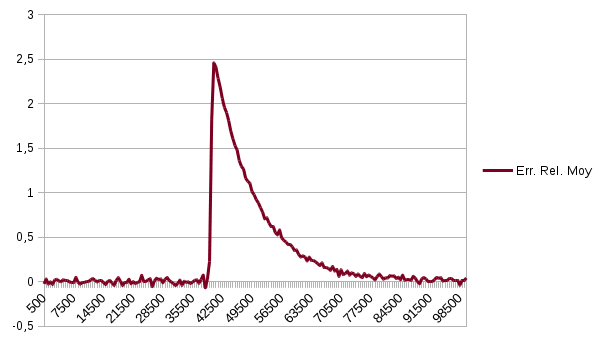
\includegraphics[scale=1]{./moy2.png}
   \caption{\label{figerr}Relative error average}
\end{figure}


\subsection{Optimizations}

We implemented MyMap in OCaml. We used the type \texttt{Bytes.t} wich
is the standard mutable byte array. The disandvantage is that we had
to rewrite a quicksort and set/get functions. We did not reach the end
of the implementations and we stopped here.


\section{Conclusion}

Organisation : nous avons développé en binôme et réalisé une part
équilibré du travail.

\subsection{Nicolas Lupinski} 
On a étudié qu'un seul problème, qui est de plus plutôt résolu. On
aurait pu se demander quels sont les autres problèmes qui admettent
des solutions astucieuses en temps linéaire et espace sous linéaire,
par exemple.  J'ai apprécié avoir à lire un article scientifique en
détail. Je n'ai pas apprécié la phase d'optimisation de
l'implémentation. Peut être à cause du choix d'Ocaml : les
optimisations de bas niveaux sont pénibles.
  

\subsection{Rémy El Sibaïe Besognet}
J'ai trouvé le sujet de l'UE plutôt intéressant tout comme sa
décomposition : approche théorique / approche pratique et
implémentation. C'était plutôt bien que tout le monde étudie le même
article, chacun apporte sa compréhension du sujet et l'exprime.

J'ai moins apprécié la deuxième partie de l'implémentation. Là où la
première demandait de programmer un concept efficace et intelligent,
les optimisations suivantes étaient plutôt basés sur des éssais en
force de brute de l'efficacité pour trouver les bons changements à
apporter. On ne retrouvait pas la démarche d'origine de l'algorithme
d'origine qui se construit sur plusieurs générations de recherche.

Je suis plutôt content malgré le résultat d'avoir pu choisir un
langage et d'avoir séléctionner OCaml qui posait plus un challenge
qu'un avantage. J'aurais aimé avoir un choix plus large de langage du
type Rust, Haskell ou des possibilités encore plus exotiques.

\bibliographystyle{plain}
\bibliography{./bibli.bib}
\end{document}

